\label{1.3.14}

\emph{Projection from a Point}

Let $\P^n$ be a hyperplane in $\P^{n+1}$ and let $P \in \P^{n + 1} - \P^n$. Define a mapping $\phi: \P^{n + 1} - \curly{P} \longrightarrow \P^n$ by $\phi(Q) = $ the intersection of the unique line containing $P$ and $Q$ with $\P^n$.

\begin{enumerate}[label=(\alph*)]
    \item Show that $\phi$ is a morphism.

    \item Let $Y \subseteq \P^3$ be the twisted cubic curve which is the image of the $3$-uple embedding of $\P^1$ (\ref{1.2.12}). If $t, u$ are homogeneous coordinates on $\P^1$, we say that $Y$ is a curve given \emph{parametrically} by $(x, y, z, w) = (t^3, t^2 u, t u^2, y^3)$. Let $P = [0 : 0 : 1 : 0]$, and let $\P^2$ be the hyperplane $z = 0$. Show that the projection of $Y$ from $P$ is a cuspidal cubic curve in the plane, and find its equation.
\end{enumerate}

\begin{proof}
    \begin{enumerate}[label = (\alph*)]
        \item We first do the particular case of $\P^n = Z(x_{n+1})$ and $P = [0 : \dots : 0 : 1]$. Let $Q \in \P^{n+1} - \curly{P}$ and let $l$ be the line connecting the two. To understand this with legitimate linear algebra, we appeal to the cone of \ref{1.2.10}. We then have lines $C(P), C(Q)$ and the plane $C(l)$ which contains both of them. All of this is, of course, in the vector space $\A^{n + 2}$. $Q \neq P$ so this is indeed a plane. Furthermore, we have the hyperplane $C(Z(x_{n+1}))$. The intersection point of $l$ and $Z(x_{n+1})$ lifts to the intersection line of $C(Z(x_n)) \cap C(l)$. Let's say $Q$ has homogeneous coordinates $[a_0 : \dots : a_{n+1}]$. Then $C(l)$ is the span of $(a_0, \dots, a_{n+1})$ and $(0, \dots, 0, 1)$. So for instance, it contains the point $(a_0, \dots, a_n, 0)$. Note that one of the $a_i$, $i \leq n$, must be nonzero as $Q \neq P = [0 : \dots : 0 : 1]$. Thus, $(a_0, \dots, a_n, 0)$ is a nonzero point in the one dimensional subspace $C(Z(x_{n+1})) \cap C(l)$. Hence, $[a_0 : \dots : a_n : 0] \in l \cap Z(x_{n+1})$ so $\phi([a_0 : \dots : a_{n+1}]) = [a_0 : \dots : a_n : 0]$. A modified version of the lemma in \ref{1.3.4} shows that this is a morphism.

        Now, we can reduce the general case to the above case. Consider a point $P \in \P^{n + 1}$ and a hyperplane $H \subseteq \P^{n+1}$ not containing $P$. Then there is a linear isomorphism $T: \A^{n + 2} \longrightarrow \A^{n + 2}$ sending $C(P)$ to the span of $(0, \dots, 0, 1)$ and $C(H)$ to the hyperplane $V(x_{n+1})$. This reduces to a linear isomorphism $\P^{n + 1} \longrightarrow \P^{n + 1}$, which we can use to appeal to the above special case.

        \item By the same logic as above, $\phi([t^3 : t^2 u : tu^2 : u^3]) = [t^3 : t^2 u : 0 : u^3]$. We of course need $[0 : 0 : 1 : 0] \notin Y$ for this to make sense. Indeed, if $[t^3 : t^2 u : t u^2 : u^3] = [0 : 0 : 1 : 0]$ then $t u^2 \neq 0$ so $t, u \neq 0$ so $t^3, t^2 u, u^3$ are all nonzero. Anyways, we want to say that $\phi[Y] \subseteq Z(x_2) = \P^2$ is a cuspidal cubic curve. The cuspidal cubic in $\A^2$ was given in \ref{1.3.2}.a as the image of $\A^1 \longrightarrow \A^2$, $t \mapsto (t^2, t^3)$. We modify this to $t \mapsto (t^3, t^2, 0, 1) \in D(x_3) \subseteq \P^2$. If we homogeneize this to a map $\P^1 \longrightarrow \P^2$ we get $[t : u] \mapsto [t^3 : t^2 u : 0 : u^3]$. The image of this is precisely $\phi[Y]$. We seek equations for this variety, and inspired by \ref{1.3.2}.a we take the homogenization of $x_1^3 - x_0^2$ and get $x_1^2 - x_0^2 x_3$.

        Certainly $\phi[Y] \subseteq Z(x_1^2 - x_0^2 x_3)$. On the other hand, take some $[a : b : 0 : d] \in Z(x_1^2 - x_0^2 x_3)$. Then we have the relation $b^3 = a^2 d$. We want to find some $[t : u]$ such that $[a : b : 0 : d] = [t^3 : t^2 u : 0 : u^3]$. If $a = 0$ then by the above relation, $b = 0$ so $[a : b : 0 : d] = [0 : 0 : 0 : 1]$, in which case we take $t = 0, u = 1$. On the other hand, suppose $a \neq 0$. Then $[a : b : 0 : d] = [a^3 : b a^2 : 0 : d a^2]$. As $b^3 = a^2 d$, this becomes $[a^3 : b a^2 : 0 : b^3]$, so we take $[t : u] = [a : b]$. Thus, $Z(x_1^3 - x_0^2 x_3) \subseteq \phi[Y] \subseteq Z(x_1^3 - x_0^2 x_3)$. Hence, $\phi[Y]$ is indeed a cuspidal cubic.

        We conclude with the plot (\ref{fig1.3.3} below) of $\phi[Y]$, which of course must be done over $\R$. We do this by taking the affine patch $D(x_3) \subseteq \P^2$ and shrinking it to an open disk in the plane $\R^2$. The boundary circle of this then represents the line at infinity $\P^1$. This is the usual CW complex structure of $\R\P^2$.

        \begin{figure}[h]
            \centering
            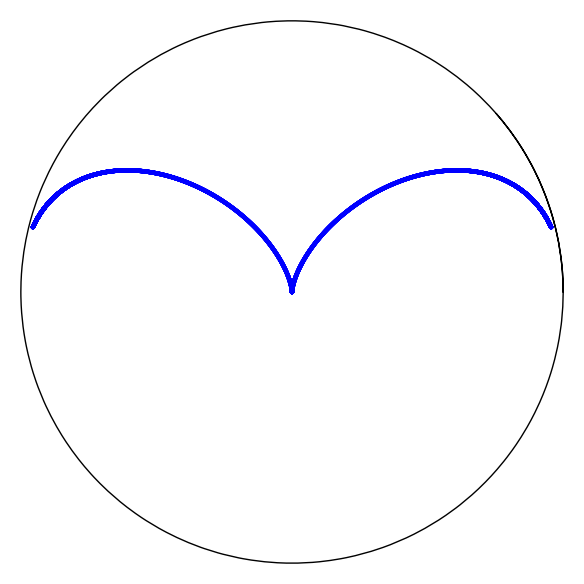
\includegraphics[scale=0.3]{cuspidal-cubic-in-p2.png}
            \caption{The cuspidal cubic in $\P^2$}
            \label{fig1.3.3}
        \end{figure}

    \end{enumerate}
\end{proof}
